\chapter{Results and Discussion}

\section{Traffic Volume Counting}

This section documents the performance of the computer vision algorithm in measuring vehicle volume. Table \ref{table:volume_table}lists the performance of the algorithm in seven pre-recorded traffic settings. Each setting is different in camera perspective, lighting conditions and traffic type and volume. More detailed descriptions and images of each traffic setting which correspond to the location ID may be found in Appendix C.1. \cite{udacity_cv} DUMMY REFERENCE

\begin{itemize}
\item\textbf{ID} An identifying number referring to each unique traffic setting location.
\item\textbf{Lane} refers to the direction of traffic that is being measured. It may be up/down or left/right.
\item\textbf{True Positive} means that a vehicle was present and correctly identified and counted (TP).
\item\textbf{False Positive} means that a vehicle was not present but one was counted anyway (FP).
\item\textbf{False Negative} means that a vehicle was present but the algorithm failed to count it (FN).
\item\textbf{True Count} is the actual number of vehicles that passed the camera node. 
\item\textbf{Precision} is the proportion of positive classifications that are actually correct, where \[Precision = \frac{TP}{TP + FP}\]
\item\textbf{Recall} is the proportion of actual positives that were correctly identified, where \[Recall = \frac{TP}{TP + FN}\]
\item\textbf{F1} is the harmonic mean of the precision and recall of the algorithm, where \[F1 = \frac{2(Precision \centerdot Recall)}{Precision + Recall}\]
\item\textbf{Accuracy} is the ratio of the true positives to the number of actual positives, where \[Accuracy = \frac{TP}{True Count}\]
\end{itemize}



\begin{table}[H]
    \centering
    \begin{tabular}{|cccccccccc|} 
    \hline
    \textbf{ID} & \textbf{Lane} & \textbf{FP} & \textbf{FN}& \textbf{TP}& \textbf{True Count}&\textbf{Precision}& \textbf{Recall}& \textbf{Accuracy} & \textbf{F1}\\
    \hline
    \multirow{3}{1em}{1}  
    &Up&0&5&41&46&100.00\%&89.13\%&89.13\%&94.25\%\\\cline{2-10}
    &Down&0&3&55&58&100.00\%&94.83\%&94.83\%&97.35\%\\\cline{2-10}
    &Total&0&8&96&104&100.00\%&92.31\%&92.31\%&96.00\%\\\Xhline{1pt}

    \multirow{3}{1em}{2}
    &Up&-&-&-&-&-&-&-&-\\\cline{2-10}
    &Down&1&4&61&65&98.39\%&93.85\%&91.18\%&96.06\%\\\cline{2-10}
    &Total&1&4&61&65&98.39\%&93.85\%&91.18\%&96.06\%\\\Xhline{1pt}

    \multirow{3}{1em}{3}
    &Up&1&3&38&41&97.44\%&92.68\%&92.68\%&95.00\%\\\cline{2-10}
    &Down&2&2&38&39&95.00\%&95.00\%&97.44\%&95.00\%\\\cline{2-10}
    &Total&3&5&76&80&96.20\%&93.38\%&95.00\%&95.00\%\\\Xhline{1pt}

    \multirow{3}{1em}{4}
    &Up&0&2&6&8&100.00\%&75.00\%&75.00\%&85.71\%\\\cline{2-10}
    &Down&0&2&8&10&100.00\%&80.00\%&80.00\%&88.89\%\\\cline{2-10}
    &Total&0&5&76&80&100.00\%&77.78\%&77.78\%&87.50\%\\\Xhline{1pt}

    \multirow{3}{1em}{5}
    &Left&0&0&8&8&100.00\%&100.00\%&100.00\%&100.00\%\\\cline{2-10}
    &Right&0&2&8&10&100.00\%&89.47\%&89.47\%&94.44\%\\\cline{2-10}
    &Total&0&5&76&80&100.00\%&92.59\%&92.59\%&96.15\%\\\Xhline{1pt}

    \multirow{3}{1em}{6}
    &Left&0&0&3&3&100.00\%&100.00\%&100.00\%&100.00\%\\\cline{2-10}
    &Right&0&1&11&12&100.00\%&91.67\%&91.67\%&95.65\%\\\cline{2-10}
    &Total&0&1&14&15&100.00\%&93.33\%&93.33\%&96.55\%\\\Xhline{1pt}

    \multirow{3}{1em}{7}
    &Left&3&0&15&15&83.33\%&100.00\%&100.00\%&90.91\%\\\cline{2-10}
    &Right&2&0&21&21&91.30\%&100.00\%&100.00\%&95.45\%\\\cline{2-10}
    &Total&5&0&36&36&87.80\%&100.00\%&100.00\%&93.51\%\\\hline

    
\end{tabular}
\caption{Traffic Volume Count Evaluation Metrics}
\label{table:volume_table}
\end{table}
\raggedbottom

\begin{table}[H]
\centering
\begin{tabular}{|ccccc|}
    \hline
                    &\textbf{Precision}&\textbf{Recall}&\textbf{Accuracy}&\textbf{F1}\\\hline
    \textbf{Average}&97.48\%&91.95\%&91.74\%&94.40\%\\\hline
    \textbf{Median}&100.00\%&93.33\%&92.59\%&96.00\%\\\hline
\end{tabular}
\caption{Average and Median Evaluation Metrics for Traffic Volume Counting.}
\label{table:averages}
\end{table}

\subsection{Strengths}

The system tests were conducted in a range of settings with different lighting and camera perspectives which lends credibility to the system's versatility and dynamism. The system is able to perform in different scenarios because it can be calibrated to accommodate different traffic scenario features, like perceived vehicle size, lighting conditions and camera angle. The computer vision algorithm's versatility is pairs well with the modularity of the system hardware. 

The algorithm is not limited to vehicle's of any one type or size as it does recognise objects according to those parameters but according to movement. Though the algorithm primarily relies on movement for detection if ta vehicle stops completely or is moving slowly this does not cause the algorithm to fail as when the vehicle commences movement it will be once again detected and counted.

\subsection{weaknesses}

The current iteration of the system cannot handle night-time situations very well because often the light cast by headlights generates an foreground blob in addition to the car that owns the headlights generating false positives. This is the cause for the high number of false positives observed at Location 7 of table \ref{table:volume_table} which was a night-time scenario. 

The system's largest weakness is when vehicles are partially or fully occluded by another vehicle, this scenario most often occurs with a camera setup whose angle of perspective is not high enough. This results in poor object separation causing blobs generated by distinct vehicles to become singular super-blob as in Figure \ref{fig:superblob}. The large proportion of false negatives at Location 4 (see table \ref{table:volume_table}) was the result of a low camera angle generating \q{super-blobs}. This phenomenon can occur in any scenario where the camera angle is not looking down onto the road it's measuring. Location 7 which had a high angle and so was immune to this and so had no false negative. The optimal optimal camera setup to avoid occlusion and blob merging is where the camera is looking down onto the roadway.

\begin{figure}[H]
    \centering
     \begin{subfigure}[b]{0.45\textwidth}
        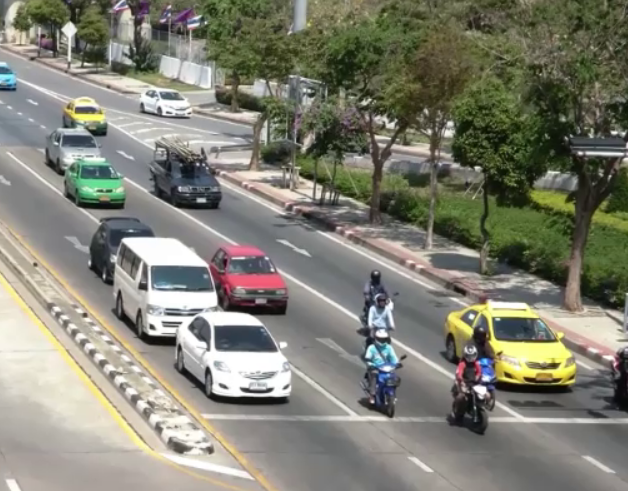
\includegraphics[width=\textwidth]{results/weaknesses/superblob}
	\captionsetup{format = hang}
    \caption{Cluster of motorbikes from Location 4}
    \end{subfigure} 
    \begin{subfigure}[b]{0.45\textwidth}
        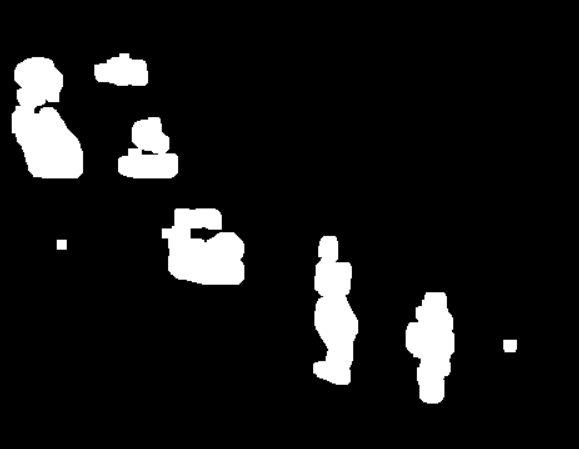
\includegraphics[width=\textwidth]{results/weaknesses/superblob_mask}	
	\captionsetup{format = hang}
    \caption{Blob of motorbike cluster at Location 4}
    \end{subfigure}
    \captionsetup{format = hang}
    \caption{Super-blob formation due to poor object separation.}
    \label{fig:superblob}
\end{figure}

The system also has some sensitivity to camera movement as when the entire camera moves it appears to the Gaussian Mixture Model that there are foreground pixels everywhere. Locations 4 and 6 suffered from some camera jostling which causes false positives and negatives. This can easily be avoided by securing the camera well but might be an issue if a node is mounted to a flexible object in a high wind area.

